\documentclass[xcolor=x11names, compress]{beamer}

%% packages
\usepackage{graphicx}
\graphicspath{{graphics/}}
\usepackage{hyperref}

%% hyperlinks
\hypersetup{
	colorlinks=true,
	linkcolor=blue,
	filecolor=blue,      
	urlcolor=blue,
	citecolor=blue
}

\begin{document}
	\begin{frame}
		\begin{center}
			\textbf{Intended Research Q:} Is an artificial minimal ecosystem possible to stay in dynamic equilibrium?
		\end{center}
	Target model\\
		\begin{figure}[h]
			\centering\includegraphics[width=\linewidth]{cycle_full.pdf}
		\end{figure}
	\begin{flushright}
		PokMan HO (CID: 01786076)
	\end{flushright}
		Image source \href{https://biologyeducare.com/difference-between-mitochondria-and-chloroplast/}{here}
	\end{frame}

	\begin{frame}
		\begin{center}
			\textbf{Intended Research Q:} Is an artificial minimal ecosystem possible to stay in dynamic equilibrium?
		\end{center}
	Alternative model\\
		\begin{figure}[h]
			\centering\includegraphics[width=\linewidth]{cycle_tgt.pdf}
		\end{figure}
		Image source \href{https://biologyeducare.com/difference-between-mitochondria-and-chloroplast/}{here}
	\end{frame}

	\begin{frame}
		Intended input (all in SI Units):
		\begin{itemize}\itemsep5pt
			\item Electromagnetic radiation intensity (a spectrum of light)\\
			\item Mg$^{2+}$\\
			\item Fe$^{2+}$\\
			\item ...
			\item all chemical ingredients are recorded in relative molar ratio (e.g. 2:9:1)
		\end{itemize}
		Intended output in csv file (all in SI Units):
		\begin{itemize}\itemsep5pt
			\item eqm time\\
			\item population of the three components (i.e. chloroplasts, mitochondria, primitive detritivores) at end time\\
			\item sugar yield\\
			\item free ATP yield\\
		\end{itemize}
	\end{frame}

	\begin{frame}
		\begin{center}
			\textbf{Intended Population Visualization}
		\end{center}
		(Sorry for copying graphs only)\\
		\begin{figure}[h]
			\centering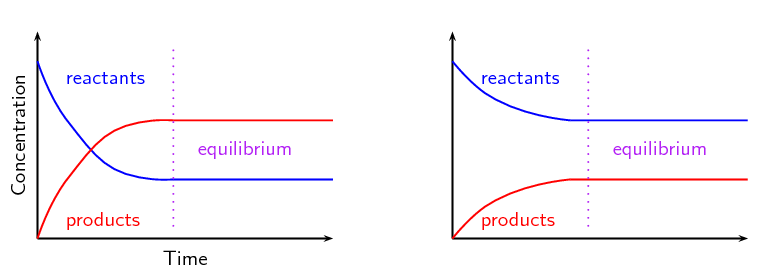
\includegraphics[width=\linewidth]{eqm_graph.png} %% all graphics must have visible name == name typed here
		\end{figure}
		Image source \href{https://www.siyavula.com/read/science/grade-12/chemical-equilibrium/08-chemical-equilibrium-03}{here}
	\end{frame}

	\begin{frame}
		Project targets:
		\begin{itemize}\itemsep10pt
			\item Which components are suitable for this minimal ecosystem\\
			\item What are needed as initial ingredients\\
			\item How much initial ingredients are needed\\
			\item What is the probability for achieving eqm if right set of raw ingredients are given\\
			\item What is the mean time for achieving (first) eqm state\\
			\item What is the eqm state for this minimal ecosystem
		\end{itemize}
	\end{frame}

	\begin{frame}
		Model assumption:
		\begin{itemize}\itemsep10pt
			\item all materials are freely-accessible to all components\\
			\item constant bio-chemical / evolutionary states for all components\\
			\item constant energy input\\
			\item stable external environment\\
			\item no phenotypic plasticity\\
			\item no other physical growth limitations except raw ingredients
		\end{itemize}
	\end{frame}
\end{document}